\documentclass[12pt, twoside]{article}
\input{../preamble}

\fancyhead[LO]{La Scuola d'Italia / Dr.\ Huson / IB Math \\* 27 April 2026}
\fancyhead[RO]{\fbox{\begin{minipage}{6cm}\footnotesize First \& Last name:\\[0.5cm]\end{minipage}}}
\fancyfoot[C]{\thepage}

\begin{document}
\subsubsection*{7.3 Classwork: Graphs of Logarithmic Functions (no calculator)}

\begin{enumerate}[itemsep=0.5cm]

%--- Problem 1: Warmup --- evaluate logs (integers + variables) [8 marks] ---
\item[1.] \textbf{Warmup}

\textbf{(a)} Evaluate each of the following.

\begin{enumerate}[label=(\roman*), itemsep=1cm]
  \item $\log_4 32$
  \vspace{0.6cm}

  \item $\log_8 4$
  \vspace{0.6cm}

  \item $\log_{1/2} 8$
  \vspace{0.6cm}

  \item $\log_3 \sqrt[3]{9}$
  \vspace{1cm}
\end{enumerate}

\textbf{(b)} Let $a > 1$ and $b > 0$. Write each expression in terms of
$\log_a b$.

\begin{enumerate}[label=(\roman*), itemsep=1cm]
  \item $\log_a (a^2 b)$
  \vspace{0.6cm}

  \item $\log_a \!\left(\dfrac{b}{a}\right)$
  \vspace{0.6cm}

  \item $\log_a \sqrt{a\, b^3}$
  \vspace{0.6cm}

  \item $\log_{a^2} b$
  \vspace{0.6cm}
\end{enumerate}

\newpage

%--- Problem 2: Inverse relationship and reflection across y = x ---
\item[2.] \textbf{The logarithm as an inverse}

You know that $y = \log_2 x$ is the inverse of $y = 2^x$. The graph of an
inverse function is the reflection of the original across the line $y = x$.

The line $y = x$ is shown below (dashed) on the axes provided.

\begin{center}
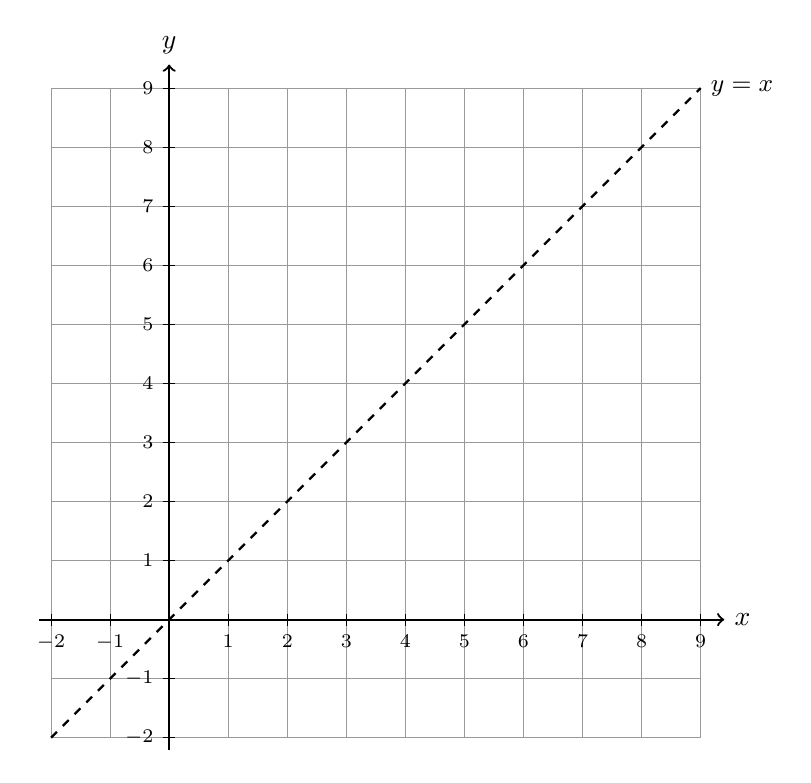
\begin{tikzpicture}[scale=0.75]
  % grid
  \draw[very thin, gray!80] (-2,-2) grid (9,9);
  % axes
  \draw[->, thick] (-2.2,0) -- (9.4,0) node[right] {$x$};
  \draw[->, thick] (0,-2.2) -- (0,9.4) node[above] {$y$};
  % tick labels
  \foreach \x in {-2,-1,1,2,3,4,5,6,7,8,9}
    \draw (\x,0.1) -- (\x,-0.1) node[below, font=\scriptsize] {$\x$};
  \foreach \y in {-2,-1,1,2,3,4,5,6,7,8,9}
    \draw (0.1,\y) -- (-0.1,\y) node[left, font=\scriptsize] {$\y$};
  % y = x line, dashed
  \draw[dashed, thick] (-2,-2) -- (9,9) node[right, font=\small] {$y = x$};
\end{tikzpicture}
\end{center}

\textbf{(a)} On the axes above, sketch and label the graph of $y = 2^x$. Mark and label its $y$-intercept. Write down the equation of the horizontal asymptote.

\textbf{(b)} On the same axes, sketch the graph of $y = \log_2 x$. Label
it, and show its $x$-intercept and vertical asymptote, labeling it with its equation.

\textbf{(c)} Complete the table.

\vspace{0.3cm}

\begin{center}
\renewcommand{\arraystretch}{1.8}
\begin{tabular}{| l | c | c |}
\hline
 & Domain & Range \\
\hline
$y = 2^x$ & \hspace{4cm} & \hspace{4cm} \\
\hline
$y = \log_2 x$ & & \\
\hline
\end{tabular}
\end{center}

\vspace{0.4cm}

\textbf{(d)} The point $(3, 8)$ lies on $y = 2^x$. State the corresponding
point on $y = \log_2 x$.

\vspace{1.5cm}

\newpage

%--- Problem 3: Transformations of y = log_2 x ---
\item[3.] \textbf{Transformations}

The graph of $f(x) = \log_2 x$ is shown below, passing through $(1, 0)$,
$(2, 1)$, $(4, 2)$, and $(8, 3)$, with vertical asymptote $x = 0$.

\begin{center}
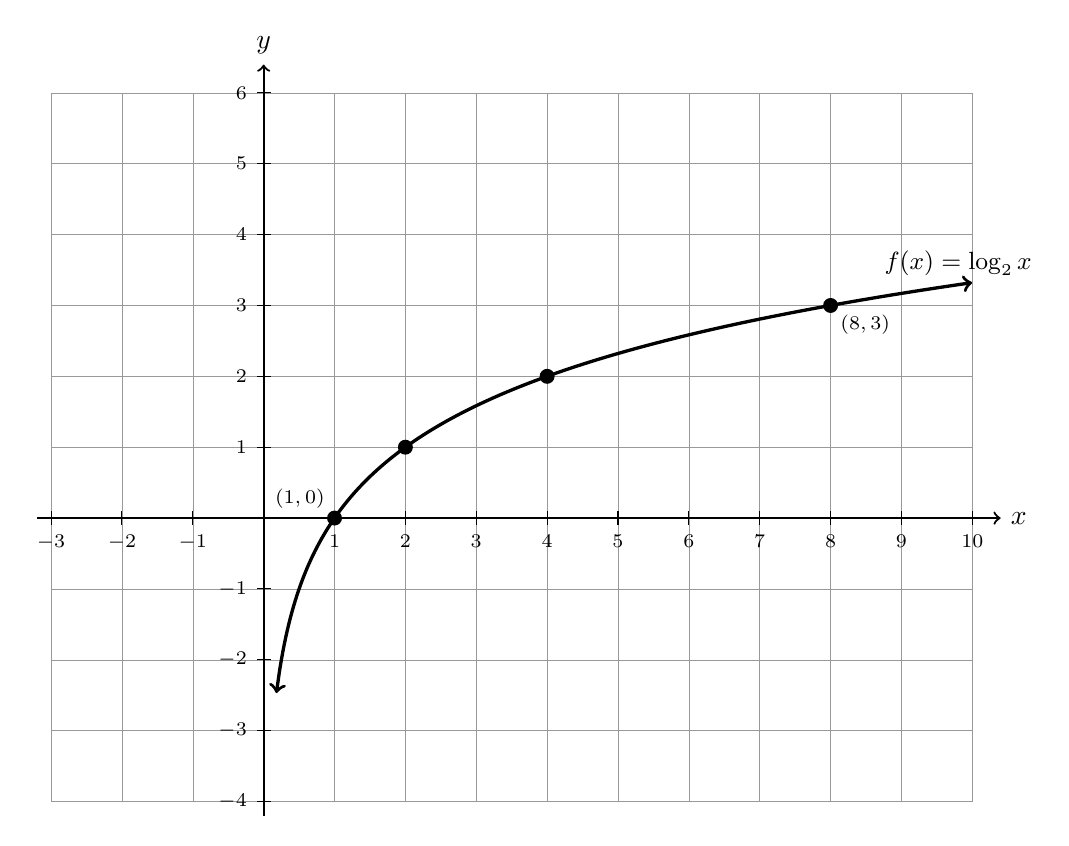
\begin{tikzpicture}[scale=0.9]
  % grid
  \draw[very thin, gray!80] (-3,-4) grid (10,6);
  % axes
  \draw[->, thick] (-3.2,0) -- (10.4,0) node[right] {$x$};
  \draw[->, thick] (0,-4.2) -- (0,6.4) node[above] {$y$};
  \foreach \x in {-3,-2,-1,1,2,3,4,5,6,7,8,9,10}
    \draw (\x,0.1) -- (\x,-0.1) node[below, font=\scriptsize] {$\x$};
  \foreach \y in {-4,-3,-2,-1,1,2,3,4,5,6}
    \draw (0.1,\y) -- (-0.1,\y) node[left, font=\scriptsize] {$\y$};
  % y = log_2 x curve, sampled
  \draw[<->,very thick, domain=0.18:10, samples=200, smooth]
    plot (\x, {ln(\x)/ln(2)});
  % key points
  \foreach \pt in {(1,0),(2,1),(4,2),(8,3)}
    \fill \pt circle (3pt);
  \node[above left, font=\scriptsize] at (1,0) {$(1,0)$};
  \node[below right, font=\scriptsize] at (8,3) {$(8,3)$};
  \node[font=\small] at (9.8,3.6) {$f(x)=\log_2 x$};
\end{tikzpicture}
\end{center}

On the axes above, sketch each of the following. Label each curve and
state the equation of its vertical asymptote.

\textbf{(a)} $g(x) = \log_2(x - 2)$ \hfill asymptote: \rule{4cm}{0.4pt}

\vspace{0.6cm}

\textbf{(b)} $h(x) = \log_2 x + 3$ \hfill asymptote: \rule{4cm}{0.4pt}

\vspace{0.6cm}

\textbf{(c)} $k(x) = -\log_2 x$ \hfill asymptote: \rule{4cm}{0.4pt}

\vspace{0.8cm}

\textbf{(d)} For part (a), state the new $x$-intercept.

\vspace{0.8cm}

\textbf{(e)} $f(a) = \frac{1}{4} $. Write down the value of $a$. Mark this point on the graph of $f$ as an ordered pair.

\newpage

%--- Problem 4: Identify base from graph + find equation from features ---
\item[4.] A logarithmic curve $y = \log_b x$ passes through the point
$(27, 3)$.

\textbf{(a)} Find the value of the base $b$.

\vspace{2.2cm}

\textbf{(b)} State the coordinates of the point where this curve crosses
the $x$-axis.

\vspace{1.8cm}

%--- Problem 5: Synthesis: equation of a transformed log graph ---
\item[5.] The graph of $y = \log_3(x - h) + k$ has vertical asymptote
$x = 2$ and passes through the point $(5, 4)$.

\textbf{(a)} State the value of $h$.

\vspace{1cm}

\textbf{(b)} Find the value of $k$.

\vspace{2.2cm}

\textbf{(c)} Sketch the graph. Mark and label the vertical
asymptote and the point $(5, 4)$.

\begin{center}
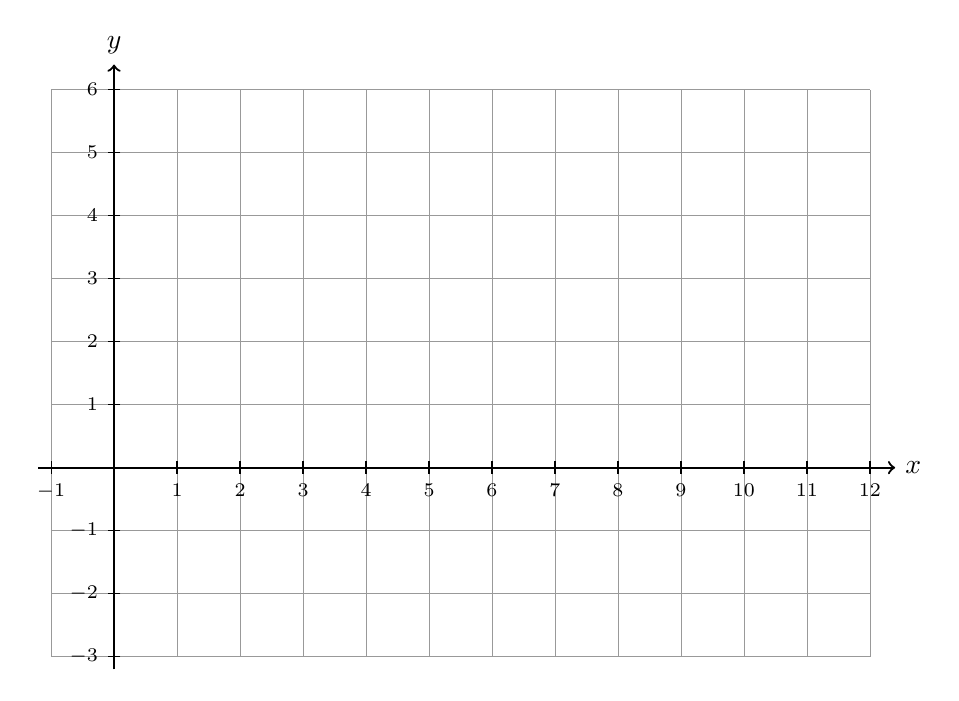
\begin{tikzpicture}[scale=0.8]
  \draw[very thin, gray!80] (-1,-3) grid (12,6);
  \draw[->, thick] (-1.2,0) -- (12.4,0) node[right] {$x$};
  \draw[->, thick] (0,-3.2) -- (0,6.4) node[above] {$y$};
  \foreach \x in {-1,1,2,3,4,5,6,7,8,9,10, 11, 12}
    \draw (\x,0.1) -- (\x,-0.1) node[below, font=\scriptsize] {$\x$};
  \foreach \y in {-3,-2,-1,1,2,3,4,5,6}
    \draw (0.1,\y) -- (-0.1,\y) node[left, font=\scriptsize] {$\y$};
\end{tikzpicture}
\end{center}

\end{enumerate}
\end{document}
